\chapter{Implementation}
\label{ch:implementation}
In this chapter we would like to walk the reader through the process of implementing 
the proposed system. Naturally, one of the~possibilities was to implement a~completely new system, 
which would comply with our requirements. But since we participate on a development of a~large RDF
application -- Payola; and based on the facts from
Section~\ref{why-payola}, we had decided to implement the proposed system as a~plugin
for Payola. This will affect the~implementation by fetching into specifications a few non--functional
requirements.

Before we start, let us mention again some tools whose authors decided to do the~
same --- to integrate them into a~larger project. We are talking specifically about 
OLAP2DataCube(Section~\ref{olap2dc}) and CubeViz (Section~\ref{cubeviz}),
which are based on the~OntoWiki platform developed by 
the AKSW~\cite{aksw} group at the~University of Leipzig~\cite{leipzich-uni}.

We would now like to describe in detail the process of integration of our proposed system with
Payola. However at first, we need to provide a description of Payola internals, thus presenting all
the facts that we deem necessary, in order to make the implementation fully understandable to
the reader.

\section{Integration of the proposed system}
We will build up on the brief description from Chapter~\ref{ch:payola} and familiarize the reader
more with the architecture of Payola. We will especially
focus on those parts that were important to the integration of the proposed system.

Payola is a web application. It is built on top of a Scala MVC framework (Play! 2.1~\cite{playfw}).
Payola takes advantage of
some modern web technologies like HTML5 (especially the canvas element).
Therefore, we will implement the system as a component of a web application.
We could have implemented the tool as a standalone 
application (e.g. a console or web a service) with a certain kind of API,
but that would have meant less than full advantage of some of the Payola framework features.
It would not allow us to profit from all the benefits described in Section~\ref{why-payola}. 

\emph{We are used to talk about Payola as either an application or a tool or a framework. To
distinguish those terms we consider Payola to be an application (or a tool) from the user’s
point of view whereas we are looking at it as a framework from the developer’s side.}

As described in Section~\ref{why-payola}, the most beneficial way of 
implementing the proposed system into Payola is as an analytical plugin. In Chapter~\ref{ch:payola}
we have got the reader acquinted with the 
general principles of how the analyses and plugins work. We have also provided some examples 
of already existing plugins. We are about to widen the variety of plugins and 
introduce a new one.

\section{Analytical plugins}
Before moving forward, one needs to understand the technical 
details behind the analytical plugins. We have already stated that such a plugin is 
a computation unit. Its task is to transform the input graph(s) into one output 
graph. The transformation fully depends on the implementation of such a 
plugin. Each plugin has always exactly one output but may have infinite number of 
inputs. It might also have no input at all. For instance, all the data 
source plugins that fetch data from some kind of storage, are generally considered to be
graph generators. That is why they have no inputs. The Filter 
plugin filters the input graph by applying a specified constraint. That is why it 
has one input (the constraint is applied on a single graph).
An example of a plugin with more than one input is known as the~\textt{Union} 
plugin, which takes two graphs and combines them together.

One can see that this is perfectly suitable for completing our task --- we are about to 
implement a system that will transform an input graph into a different one.

In the case of the~texttt{Filter} plugin, we spoke about \emph{specifying a 
constraint}. The plugin has parameters that enable its reuse in multiple--case scenarios. For instance,
the Data Fetcher plugin has a parameter, which tells 
the plugin where to fetch the data from. It would be to no avail had we implemented a plugin
enabling the user to fetch the data solely from DBPedia (the fact that it is one of the largest data
sources notwithstanding).
The original implementation of Payola recognized 4 different types of plugin 
parameters --- \texttt{string}, \texttt{float}, \texttt{int} and \texttt{boolean}. 

If the reader were to remember Chapter~\ref{ch:proposal}, they would recall that we determined that 
the system would need the following input:
\begin{itemize}
  \item An arbitrary RDF graph.
  \item A graph containing the DCV data structure definition.
  \item A transformation pattern.
\end{itemize}

At this point we should decide, which of them would become parameters and which of 
them inputs of the plugin. It may seem to be a good idea to supply the 
graphs as inputs and the transformation pattern as a parameter. At least, it is 
consistent with the idea that a graph is an input type of an analytical plugin. 
But if we think about it just a bit longer we realize that once we have the 
transformation SPARQL query, we do not need the data structure definition for 
processing anymore. We just need the plugin to receive the input data and transform 
them while applying the transformation query.

We need from the data structure definition to only inform the user as to what kind of data are they 
are working 
with. We require them to select a valid and meaningful pattern. 
Therefore, we need for the plugin to have one input (the arbitrary RDF dataset) and 
one parameter (the transformation pattern). Under normal circumstances
that would be sufficient, but we 
need to find a way of storing the data structure definition metadata in order 
to present them to the user if necessary.

When we started experimenting with the system, the idea of specifying the 
transformation pattern was a little bit different. Initially, we thought that it 
would be possible to specify a pattern for each DCV component separately. After 
a while, we had learned that it makes the task harder for the user. It is more complicated to select a 
valid pattern, especially when the pattern needs to be a connected graph for a conclusive expression
of the relations between matched entities.

In the process of experimenting, we came up with a new way of storing the 
data structure definition within an analytical plugin. We made each component to 
be a parameter in order to enable the user to select a pattern for each of 
them. Such an approach was an unexplored territory in the scope of the Payola framework.

\begin{figure}
	\centering
	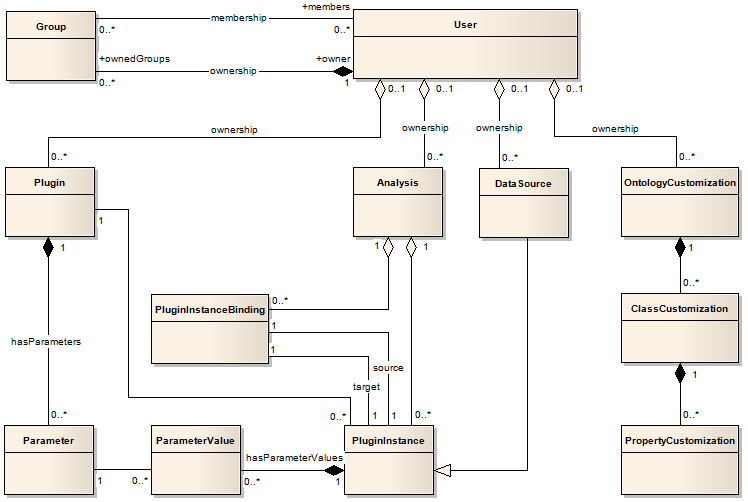
\includegraphics[width=140mm]{img/params-schema.png}
	\caption{Payola entities schema containing a schema of the parameters 
	subsystem of the Payola framework.~\cite{payola:dg}}
	\label{fig:params-schema}
\end{figure}

The architecture of the parameters subsystem can be deduced
from a schema in Figure~\ref{fig:params-schema}. We distinguish between two 
different basic types of entities -- \texttt{Plugin} and \texttt{PluginInstance}. The first 
one represents a template for each plugin type. An instance of the second one is created for
each occurrence of the plugin in an analytical pipeline. Whilst an instance of the \texttt{Plugin}
class defines the number of parameters, an instance of the \texttt{PluginInstance} 
defines their values.

For instance, the Filter plugin implementation is coded in the class \texttt{Filter}.
That class is derived from the \texttt{Plugin} abstract class. There is a single record in the database table
\texttt{plugins}, which represents the information about the Filter plugin existence.
Among others, it contains the FQDN of the \texttt{Filter} class. This course will inform the analytical
pipeline evaluator which class is responsible for handling
a specific type of plugin. The class also defines that the Filter plugin has 3 parameters. It even 
defines their data types. One single instance of such a class is sufficient. On the other hand, we need
multiple instances of the \texttt{PluginInstance} class in order to
handle parameters values. Each occurrence of the Filter plugin will be probably 
used with a completely different set of parameters (while having the same count).

\begin{figure}
	\centering
	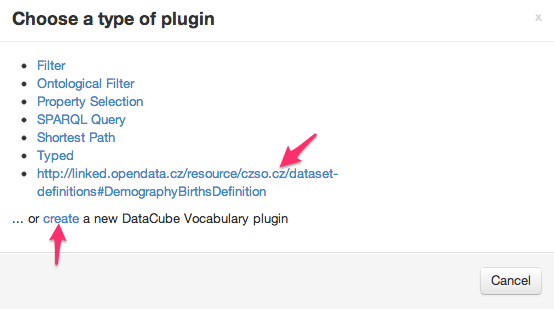
\includegraphics[width=100mm]{img/choose-plugin.png}
	\caption{A user is able to create a new DCV plugin or to connect an existing one.}
	\label{fig:choose-plugin}
\end{figure}

The aforementioned features enabled us to implement what is shown in 
Figure~\ref{fig:choose-plugin}. When adding a new connection into the analytical 
pipeline the user is able to create a new DCV plugin or connect an existing one. 
To create a new one, the user is required to supply an URL of a graph containing 
a chosen vocabulary (see Figure~\ref{fig:create-plugin}). After processing the 
supplied graph, the user is required to choose a desired definition as shown in 
Figure~\ref{fig:choose-def}.

\begin{figure}
	\centering
	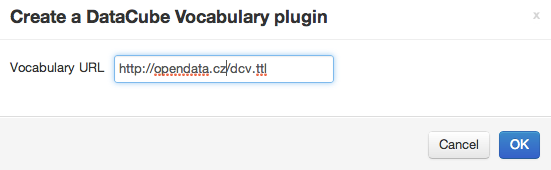
\includegraphics[width=100mm]{img/create-dcv.png}
	\caption{To create a new one, the user is required to supply an URL of a graph containing 
a chosen vocabulary.}
	\label{fig:create-plugin}
\end{figure}


\begin{figure}
	\centering
	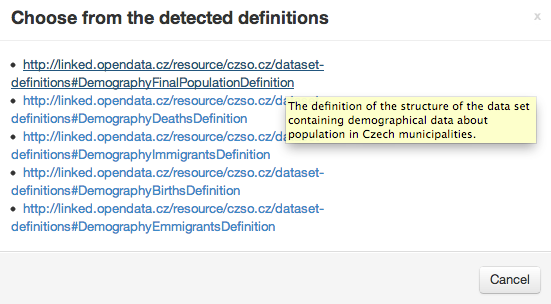
\includegraphics[width=100mm]{img/choose-def.png}
	\caption{A list of detected DCV definitions is shown to the user.}
	\label{fig:choose-def}
\end{figure}

\subsection{Data Cube Vocabulary analytical plugin}

\begin{figure}
  \begin{verbatim}
/**
  * @param _name Name of the plugin.
  * @param _inputCount Count of the plugin inputs.
  * @param _parameters The plugin parameters.
  * @param id ID of the plugin.
  */
abstract class Plugin(
    protected var _name: String,
    protected val _inputCount: Int,
>    protected val _parameters: immutable.Seq[Plugin#ParameterType],
    override val id: String = IDGenerator.newId) ...
  \end{verbatim}
  \caption{The header of the \texttt{cz.payola.domain.entities.Plugin} class. It does not restrict the count
  of the passed parameters, it receives a generic sequence.}
  \label{fig:plugin-trait-code}
\end{figure}

In the case of the implemented plugin, we take advantage of the fact that the 
\texttt{Plugin} abstract class allows us to pass a variable count of parameters to the 
plugin implementation. See Figure~\ref{fig:plugin-trait-code} to learn how the abstract class header 
looks like. That is beneficial mostly due to every vocabulary being consisted of a 
different count of components. But we need to create an instance of the \texttt{Plugin} entity
for each vocabulary in order to store the components metadata.

Until now, there was usually just one entity derived from the type \texttt{Plugin} associated with
a codebase of a plugin. The concept of plugins was not formerly designed to have
a variable count of parameters for each plugin instance.

That is why we have decided to acquire a new approach. By adding a plugin 
into the analytical pipeline we will give the user an opportunity to create a 
new instance of the \texttt{Plugin} class. This instance is based on a specified data structure definition
with an appropriate count of parameters. Each parameter represents a component 
of the data structure definition. Moreover, a \texttt{Plugin instance} is instantly created 
based on the formed \texttt{Plugin} template. A representation of that instance is consequently 
rendered into the pipeline editor and the instance itself bound into the 
analytical pipeline.

\begin{sloppypar}
Let us present a short example and consider an exemplary data structure definition \texttt{example:population}
consisted of 3 
components; let us say dimensions \texttt{example:refArea}, \texttt{example:populationAsOf}
and measure \texttt{example:populationCount}. Such a data structure leads us to 
the creation of a new plugin of type Data Cube Vocabulary named 
\texttt{example:population}. It would have 3 parameters named in the same way the 
components are, all of type \texttt{string}.
\end{sloppypar}

Such an implementation fits into the Payola architecture. Moreover, as a side--effect, it brings
an added value --- based on the data structure definition, a plugin is created. 
That means that there will be a specific plugin for each DCV data structure 
definition. That plugin can be owned by the user who initiated its creation. 
From that point onward, the plugin will be available to the user and they
will not need the data structure definition anymore. What we got is a 
component, which is reusable on the level of an analyzer. Since the user is able to 
share their custom plugins with other Payola users, they are
naturally able to share the created Data Cube Vocabulary plugin, too. 

An important fact is that regardless of the amount of the parameters, it is sufficient 
to have a single codebase. We will implement a single Scala class that represents the behaviour 
of the plugin. That is because the \texttt{Plugin} abstract class (fig.~\ref{fig:plugin-trait-code})
from the Payola framework
API does not constrain the count of parameters supplied to the class.

This however causes a different kind of a problem. As we have stated before, the 
approach to selecting a pattern per each component does not align well with what we 
need. Only a few lines above we also discovered that all that is needed is a 
single parameter --- a transformation pattern. Therefore, we need to modify a bit the 
behaviour of the analytical pipeline editor in order to render the \texttt{Plugin instance}
in a non--generic way. We will also coerce the plugin to always store the transformation query 
within the first parameter.

We realize that this approach is not quite clean nor nice but we need to accept it for several reasons.
The first being a simultaneous research based on the original Payola done by various people where
at the time of writing this thesis and experimenting with the proposed system, some of the researchers 
would not be able to overcome the major architectural change and thus not finishing their project.
But such a change would have been required since 
it would have been necessary to introduce a new parameter into the \texttt{Plugin} trait. 
It would demand something general enough to carry metadata that are not determined for 
computational purposes (and distributed together with the plugin throughout the whole system).
It would have also been extremely difficult to coordinate such 
a change at that time that is why it will be more suitable to refactor the 
implementation in the future when the concept of the proposed system is 
proved.

\begin{figure}
	\centering
	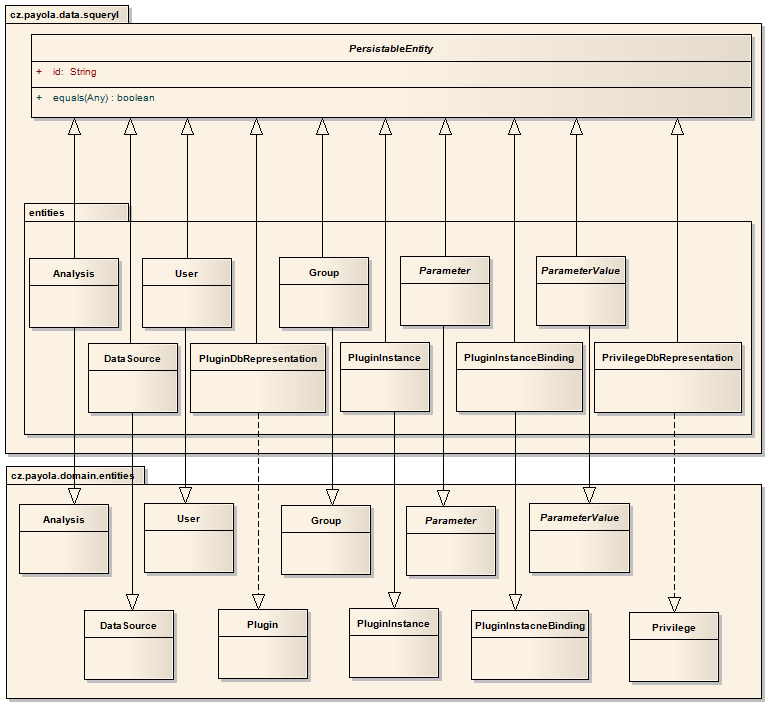
\includegraphics[width=140mm]{img/data_entities.png}
	\caption{The data access is divided into 3 layers. The first one, which is a part of
	the common package defines entities and relations between them (not in the figure ---
	see Figure~\ref{fig:packages-structure}).
	The second one is a part of the domain package. It defines basic business logic.
	The last one has its own package --- data. It binds the others with a concrete DAL
	implementation, in this case with the Squeryl ORM. ~\cite{payola:dg}}
	\label{fig:3-layers}
\end{figure}

The second reason is that the Payola data access layer is consisted of three different sublayers
(Figure~\ref{fig:3-layers}) and 
due to the utilization of the Squeryl ORM framework~\cite{squeryl}, it would be a very difficult 
task to try and modify the existing database structure. In the list of the future changes of 
the Payola framework there is a thought for a replacement of the underlying ORM framework
and respectively for a 
heavy refactoring of the data access layer.

Therefore, we have decided to focus on the task and implement the feature with 
as little modifications to the Payola framework as possible. In fact, the used adjustment is
kept in the socpe of the newly added features and does not blemish the rest of the framework.

The implementation of the plugin is pretty straightforward since we are 
taking advantage of the Payola framework. The Payola framework recognizes a
special subtype of a \texttt{Plugin}, a \texttt{SparqlQuery}. There is a special 
reason for this as a SPARQL query could be executed on a remote data source, 
e.g. a SPARQL endpoint. A series of SPARQL queries could be optimized into a 
single, more efficient query. Without such a mechanism, the framework would
have to fetch all the data from the data source, transfer them to the server 
where Payola is running on, store them in the memory (wrapped with
the Payola internal object representation) and pass it to a plugin. After that, the 
graph would be processed inefficiently within the memory of the Payola server with 
the JENA RDF toolkit consuming uselessly a lot of probably unnecessary computation time. See 
Figure~\ref{fig:plugin-hierarchy} to see the whole plugins’ hierarchy.


\begin{figure}
	\centering
	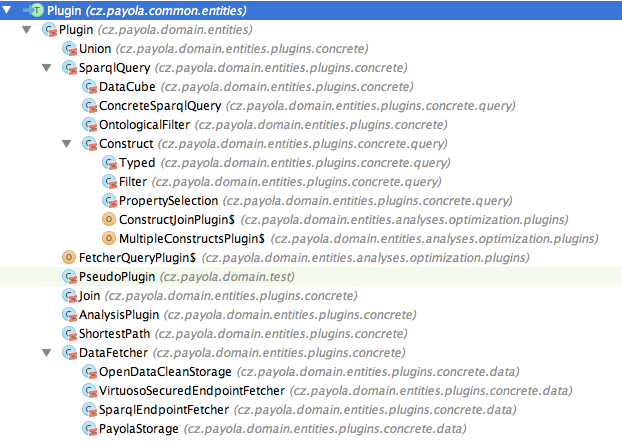
\includegraphics[width=100mm]{img/plugin-hierarchy.png}
	\caption{Payola plugin hierarchy. Notice the SparqlQuery class.}
	\label{fig:plugin-hierarchy}
\end{figure}

Moreover, the Payola framework restricts the use of a non--SPARQL--query 
in the analytical pipeline right after the data fetcher plugin. That is done in order to avoid 
the aforementioned performance difficulties. There is one restriction regarding our plugin if we
were to derive it from the \texttt{SparqlQuery} class. The complete behaviour of the plugin needs to 
be expressed by a single SPARQL query. Fortunately, such a constraint does 
comply with what we need in order to implement the proposed system. That also means
that the existing Payola query optimizer will engage and 
will make the plugin execution faster. Therefore, the system will again 
benefit from the integration with the Payola framework.

The plugin will load the stored query from the database and pass it to the 
evaluation framework, which will handle the rest.

\subsection{Obtaining the transformation pattern}
The more complicated task still awaits us. We need to implement an interface, 
which will obtain the transformation pattern from the user. The implementation 
builds up on what we have learned of the pattern in Chapter~\ref{ch:proposal}.
The best way is to simulate the 
approach we used for getting the formal expression of the transformation pattern
(see Section~\ref{sec:pattern-definition}).

We have already stated that we are about to implement a user interface, which 
will allow the user to select the pattern based on the Tabulator's (Section~\ref{sec:rw:tabulator})
query--by--example principle. But to do that, we need to introduce a lot of new 
features into the Payola framework.

\subsubsection{Analysis preview}
In order to enable the user to choose a pattern by an example, we need to offer them a preview
of the given dataset. The dataset serves as an input graph of the mapping process. 
We have decided to make the proposed system a part of the analytical 
pipeline, which brings on some interesting and unexpected complications.

Mainly, the dataset may come from any point of the analytical pipeline execution. In 
fact, we need the evaluation framework to give us a partial result. We need the 
analyzer to process the pipeline and at some point, to take an input of the 
inserted Data Cube Vocabulary Plugin instance and send it to us as a result. 
Moreover, only a part of the pipeline could be used to make a preview. For instance, if had an analysis
based on extracting the data from several different data sources, 
let's say 4, those 4 fetching processes would run collaterally regardless of the 
fact that the DCV plugin is a part of one of them. We will throw away the 
results of the rest. It is shown in Figure~\ref{fig:dcv-preview-useful}.

\begin{figure}
	\centering
	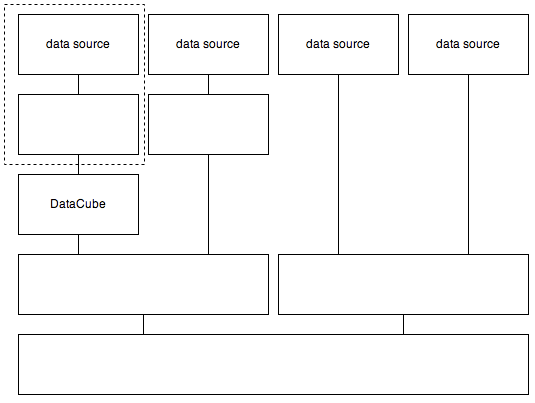
\includegraphics[width=100mm]{img/dcv-preview-useful.png}
	\caption{Making a preview for the Data Cube Vocabulary plugin. Only the plugins in
	the dashed box are relevant. The rest of the analytical pipeline is not.}
	\label{fig:dcv-preview-useful}
\end{figure}

It brings on not only a technical complication, it also rises a performance 
question. The analytical pipeline may take a lot of time to be processed.

That is why we had to introduce a mechanism, which, in the right moment, 
extracts a proper sub--pipeline. If the reader looks closer on 
Figure~\ref{fig:example-analysis} they learn that the pipeline is,
in the reverse topological order, 
a tree (as known from the graph theory). Every instance has 
one output. Every output is connected to an input of a successor (if present, if not it is an output
of the whole pipeline). Therefore, it is easy to traverse the tree and select a 
subtree, which precedes the Data Cube Vocabulary plugin instance.

Such a tree is then used in the background without the knowledge of the user to 
create a completely new analytical pipeline. When this step is complete, such a pipeline can 
be executed by a standard pipeline evaluator. That is because the result of the whole 
newly created pipeline is the dataset we make the preview from.
See an example of such a pipeline in Figure~\ref{fig:dcv-extraction}.

\begin{figure}
	\centering
	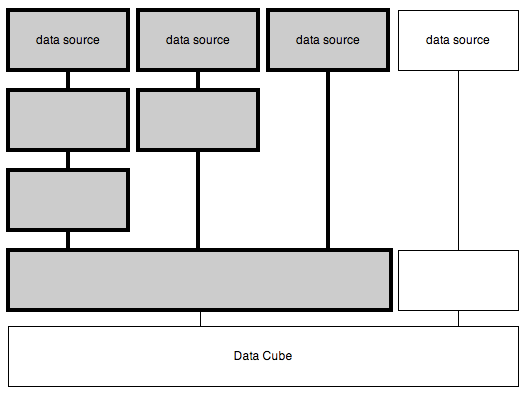
\includegraphics[width=100mm]{img/dcv-extraction.png}
	\caption{Making a preview for the Data Cube Vocabulary plugin. The highlighted
	plugins are required to be evaluated and becomes a part of a sub--pipeline created
	in the background.}
	\label{fig:dcv-extraction}
\end{figure}

Nonetheless, what remains is a potential performance problem, which is partially given 
by features provided by the Payola framework. The result of executing an 
analytical pipeline could become eventuallya very huge dataset. A dataset so 
large that it may not fit into the memory of the user's computer. That is a 
limiting factor, since the visualisation is performed fully on the client--side. 
It makes no difference whether it is a table or a graph rendered into the canvas HTML element.

In order to solve this problem in the Payola framework, a larger milestone is 
planned. The results need to be cached on the server hosting Payola.
Such an approach could be seen in the case of the project 
Explorator (section~\ref{sec:rw:explorator}) project, which implemented a local cache
while utilizing the tool SESAME~\cite{sesame}. It is planned to introduce a new 
subtype of the~\texttt{Graph} trait, ~\texttt{PersistentGraph}, which would be 
cached on the Payola server in order to enable techniques like pagination, 
exploration in the analytical mode, etc. Since this requires also a huge 
modification to the existing visualizers but is not a goal of this thesis, we will 
not realize this plan. However we will implement the preview in a way that will 
automatically take advantage of the modifications when they are done.

This still leaves us with the problem of a huge results dataset. Therefore, we 
decided to make use of the~\texttt{LIMIT} SPARQL query statement, which will 
enforce the results to be reasonably large. This could be done by 
extending the previously extracted sub--pipeline with appending a plugin that 
will limit the number of the results of the analytical
pipeline evaluation (see Figure~\ref{fig:dcv-extraction-limit}). Therefore, we 
introduced another completely new plugin -- \texttt{Limit}.

\begin{figure}
	\centering
	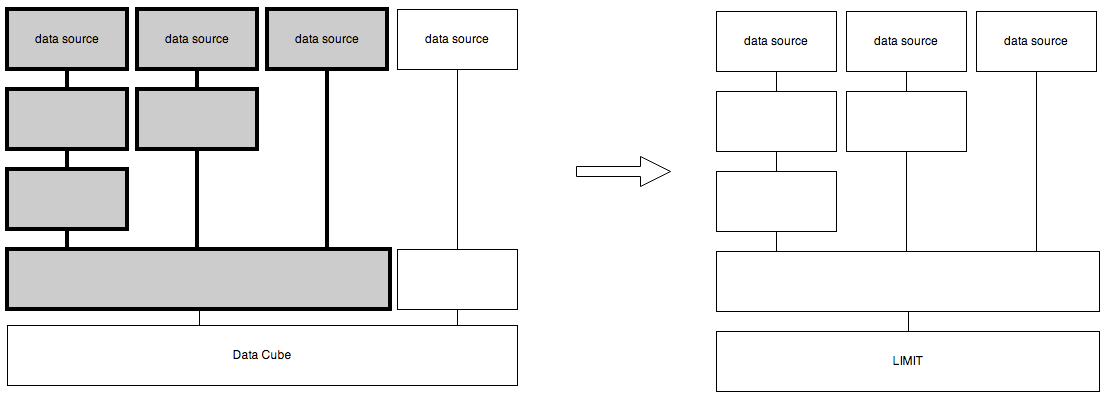
\includegraphics[width=140mm]{img/dcv-extraction-limit.png}
	\caption{Making a preview for the Data Cube Vocabulary plugin. An instance of
	SparqlQuery plugin representing a LIMIT statement is added.}
	\label{fig:dcv-extraction-limit}
\end{figure}

Unfortunately, that brings a completely new problem. By limiting the size of 
the result, it is possible that some important vertices might get excluded from the preview.
And there is no way of 
telling, which vertices could be important to the user. Therefore, we made the 
size of the preview to be a variable that could be changed before making the preview and 
selecting the transformation pattern. Of course, the better approach would be to 
insert the plugin into such an execution point of the pipeline that it would 
work with data as small as possible. In other words, we should use an analysis 
to compensate a large size of the original dataset, if possible.



\subsubsection{Obtaining the pattern}
Hopefully, it is now fully understood what it is required to be done before a preview 
is made so we can move onto the description of the way of obtaining the pattern 
from the user. Moreover, we will describe, which components and why have been 
modified or newly implemented.

\begin{sloppypar}
We take advantage of the previously presented approach (the query--by--example), which we 
consider to be the best for the user. Firstly, the user is asked to mark a vertex that represents
the first component of the associated Data Cube Vocabulary data structure 
definition. Since the only criteria we set is that the pattern needs to be a 
connected graph at any time, it is sufficient to select only a single vertex.
Of course, the user might consider selecting a more complicated pattern with keeping in mind the 
\emph{reference vertex} concept mentioned in the proposal (Chapter~\ref{ch:proposal}).
\end{sloppypar}

If we enable the user to extend the pattern not only by adding a vertex, 
which has an incoming edge from one of the already added vertices, but also by adding 
a vertex, which has an outgoing edge into one of the already added vertices, 
the user is capable of building a complicated pattern in a way compatible with a natural thinking process.
They will select the
important vertex \emph{accidentally} while extending the 
pattern in order to select another. Therefore, the only restriction 
applied in the vertex selection mode is that we prevent the user from selecting 
a non--related vertex (more accurately a vertex, which would breake the connected 
graph invariant).

The selection process is made to be as simple as possible. We will describe the 
user interface in the following text more deeply.

\subsection{User interface}
The basics of the user interface come out of the architecture of the Payola 
framework. We need to make the plugin as simple as possible for the user. But we 
also need to keep it aligned with the design of the Payola framework. In order to 
make the reader understand the following text, we need to dive a bit into the 
architecture of the Payola application.

As stated before, Payola is a web application. Its implementation is based on the MVC 
design pattern. Nowadays, that is a usual approach to a web application. However, it is not that usual 
to acquire a stance to the utilization of a design pattern on the client--side. The 
Payola team has decided to use the MVC pattern there as well and due to 
the presence of the s2js compiler, the client--side is also being developed in 
the Scala programming language.

Therefore a majority of pages produced by the Payola application is delivered 
in two different parts. The layout of a page and a placeholder for the client 
side application is rendered on the server while utilizing the subsystems of the 
Play Framework 2.x. The placeholder is then provided to a JavaScript application,
which is referenced from the rendered layout. The utilization of the s2js compiler and
the custom RPC gateway (which translates JSON calls into method invocation and serializes its results
back to the client), prevents code duplication and makes the development process more transparent.

Therefore, every client--side application can avoid becoming a confusing piece of a
spaghetti code and utilize the MVC pattern. A crucial feature is the RPC 
mechanism that, hand in hand with the s2js compiler brings a way of transparent 
client--server communication.

The analytical pipeline editor is one of those client--side MVC applications. We 
are interested specifically in this one since we require for it to be able to work 
with our newly introduced Data Cube Vocabulary analytical plugin.

Until now, the pipeline editor applied a unified approach for rendering the 
layout of the pipeline. Every plugin was rendered while using a generic 
renderer, which determined the appearance of the plugin based on its metadata. An 
example of such a rendered pipeline could be seen in
Figure~\ref{fig:example-analysis-editable}. The reader can see a rendered title, based on 
the name of the plugin and a parameter form. The form is based on the type of the 
corresponding parameters. A \texttt{string} parameter gets rendered as an input or a textarea based on
an additional flag \texttt{isMultiline}, which determines whether the value can be spread into multiple lines.
A \texttt{int} or \texttt{float} parameter is also rendered as an input field. A \texttt{boolean} parameter 
is rendered as a checkbox.

\begin{figure}
  \centering
    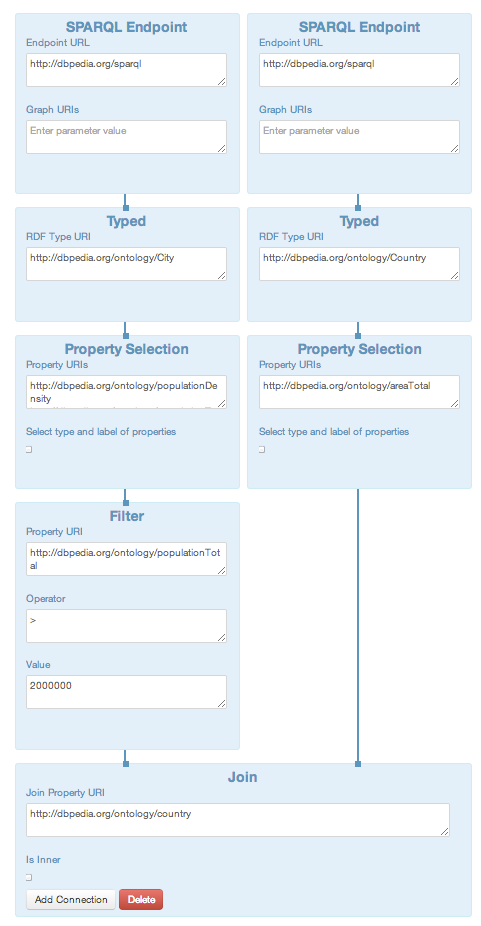
\includegraphics[width=100mm]{img/editable-analysis.png}
  \caption{An example of an editable analysis (retrieving a list of cities with a certain population size).}
  \label{fig:example-analysis-editable}
\end{figure}

Since we would like to provide the ability to select a pattern, we need to 
introduce a completely new approach. To keep it generic, we start with the 
modification of the parameters subsystem. We would like to introduce a new type 
of parameter, a \texttt{pattern}. Since the data access layer of Payola is very 
difficult to modify, we use a less obtrusive approach. A pattern results in a 
SPARQL query, which is a string. Therefore, we add a flag to the string 
parameter, called~\texttt{isPattern}, which the system will take advantage of. It 
is based on the same unobtrusive principle as the \texttt{isMultiline} flag.

Another problem comes out of the fact that a plugin has as many parameters as 
the data structure definition has components and we utilize just the first one 
to store the query. That also means that we need to render the representation 
of the plugin in a slightly different way. At the time of implementing this 
thesis, the same requirement came up from two other developers, who integrate their 
tools with Payola. Therefore, we introduced a mechanism, which solves the 
problem of loading custom plugin renderers.

We introduce a dynamic plugin instance renderer loader for an analysis editor. 
Based on the plugin classname, it tries to load a custom override of the default 
renderer. It enhances the extensibility of Payola. Until now, it was not 
possible to override the visualization of a plugin instance within the editor. The 
user was able to upload a custom analytical plugin, but they were not capable of affecting its
appearance in the editor.

\begin{sloppypar}
With our loader, the user is able to define a custom renderer derived from 
one of the \texttt{ReadOnlyPluginInstanceView} and \texttt{EditablePluginInstanceView} 
classes. The name of the override is precisely given. It is required to match one 
of the following patterns: \texttt{{classname}PluginInstanceView},
\texttt{{classname}EditablePluginInstanceView}. The implementation is required to
be declared within the \texttt{cz.payola.web.client.views.entity.plugins.custom} package.
\end{sloppypar}

The editor was altered so that it does not create renderer instances itself. It 
uses a newly introduced \texttt{PluginInstance\allowbreak ViewFactory}. This 
factory is responsible for creating a proper instance. Based on the given plugin 
classname it calls a dependency package manager. The manager is a part of the 
s2js compiler and it provides a JavaScript implementation of the required class
with all the necessary dependencies. Therefore the factory calls the manager and 
requests an implementation of a specified override. If it exists, the manager 
returns its implementation. If it does not, it returns an empty string. After 
that, the factory tries to make an instance of the override. If it succeeds, an 
instance of the override renderer is created. If it fails, it returns an 
instance of a generic renderer. 
 
Our custom implementation of the Data Cube Vocabulary plugin renderer results 
in a form shown in Figure~\ref{fig:DCV-plugin-view}. First of all, it 
enables the user to select the pattern. Clicking the Preview button starts the process of making a
sub--pipeline, evaluating it and rendering a preview. It also opens a pattern--selection
dialog, which we introduce later. The second provided field enables the user to specify how large should 
the pattern--selection preview be. We have already presented the reason behind this 
a few paragraphs above.

\begin{figure}
	\centering
	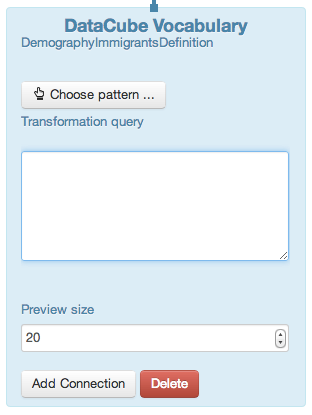
\includegraphics[width=60mm]{img/custom-dcv-piv.png}
	\caption{Data Cube Vocabulary plugin instance custom view.}
	\label{fig:DCV-plugin-view}
\end{figure}

The last part of the UI is the pattern selection dialog. After the user clicks 
on the button of the rendered plugin, the application extracts a sub--pipeline, 
which is relevant to the preview. Such a pipeline is executed
automatically. When the pipeline evaluation is done, the application opens a new 
dialog, which gives the user the opportunity to select the transformation 
pattern. With every step, the user is presented with a label and/or a URI of the 
matching DCV component based on what is available. An example of a pattern 
selection is shown in Figure~\ref{fig:pattern-selection} (some additional details are provided
in Section~\ref{sec:pattern-definition}
and in figures~\ref{fig:pattern-selection} and~\ref{fig:pattern-enhancement}).
With a single click 
the user includes a vertex into a constructed pattern. A double--click 
has it representing a currently processed component. We also had to modify the 
visualization algorithm to avoid collapsing literal vertices into a info table. 
We need the literals to remain visualized in order to be selectable.

\begin{figure}
	\centering
	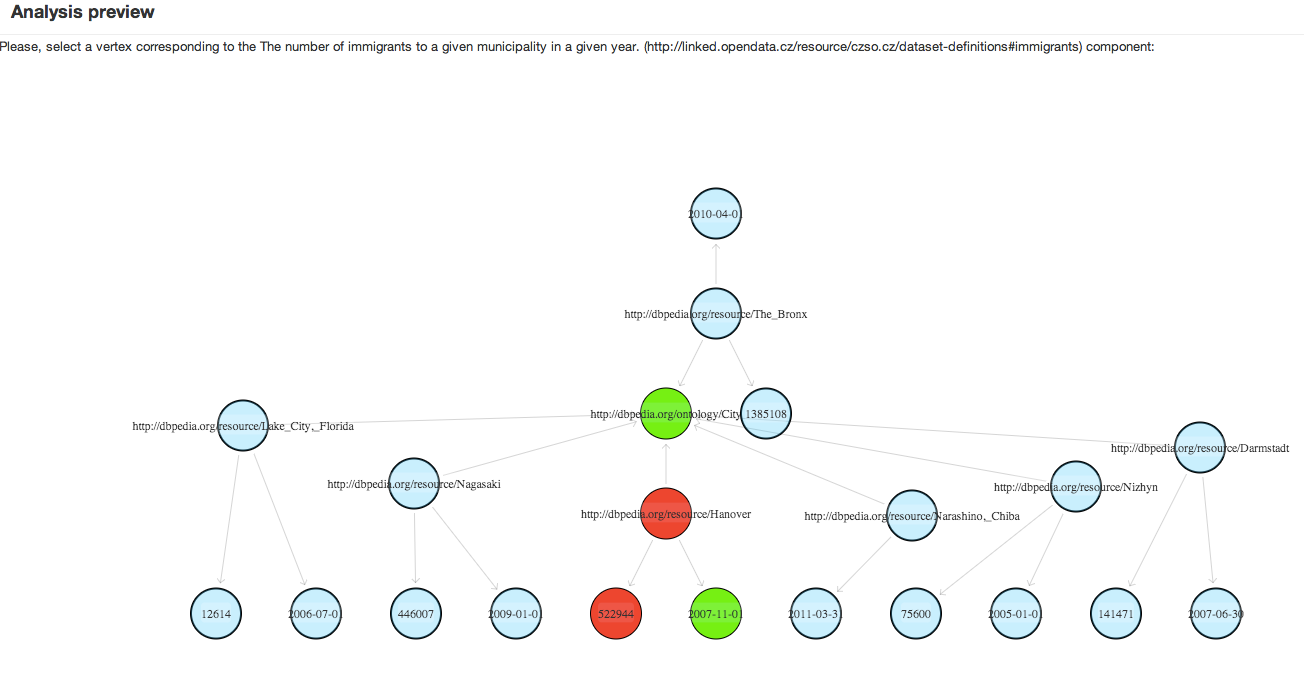
\includegraphics[width=140mm]{img/pattern-selection.png}
	\caption{An example of a pattern selection.}
	\label{fig:pattern-selection}
\end{figure}

\section{Visualisers}
As stated in Chapter~\ref{ch:proposal}, we have decided to implement two 
different visualization plugins for Payola. All the presented 
visualizers are configurable by specifying a Data Cube Vocabulary.
As in the case of the rest of the 
system, the implementation of the visualization plugins will be influenced 
by the architecture and features of the Payola framework as well.

The feature that is lacking the most  is a sophisticated faceted browsing. All the presented plugins 
implement offered filters only on the client--side, therefore all the data needs 
to be loaded within the memory of the user’s computer. As described before, Payola 
needs a series of modifications in order to work effectively with larger 
datasets, hence a client--side--only visualization is the only one currently making sense.

To make them able to work with the Data Cube vocabularies, we had to append 
definitions of those vocabularies into the result of the mapping process. The 
visualizer is then able to acquire them and take advantage of them. For instance 
while building a user interface.

\subsection{TimeHeatmap}
In order to deliver the TimeHeatmap visualizer, we took advantage of an existing 
map library. We chose to integrate a visualization based on Google Maps API. We 
decided to do so for several reasons. One of them is an easy use of the API and that it allows us to
create an eye--catching visualization in a short 
time. Google is known for its high--quality map imagery and due to its 
infrastructure also for a reliable delivery. The API also offers the ability to create a heatmap layer.

But the heatmap layer itself is not enough. In order to support the time 
dimension, we had to come up with a way of visualizing time entries. The 
interface is built with the following idea in mind. Let us imagine an example of 
population size data (see Figure~\ref{fig:impl-pop-ex}).

\begin{table}
  \begin{center}
\begin{tabular}{l|l|l}
  City & Population size & Year \\ \hline
  Prague   &    1000000   &   2010 \\
  Prague   &    1100000   &   2011 \\
  Prague   &    1200000   &   2011 \\
  Liberec   &    100000    &  2010 \\
  Liberec   &    110000    &  2011 \\
  Liberec    &   112000    &  2012
\end{tabular}
\caption{Population size example}
\label{fig:impl-pop-ex}
  \end{center}
\end{table}

It is more constructive to visualize such a dataset year--by--year. Grouped values are 
not very attractive no matter what aggregation is applied. The most useful 
approach is to enable the user to make a slice based on the year and visualize a 
heatmap for the selected year.

Therefore, we wrap the map with a custom control. It contains a list of years 
detected in the dataset. The user is able to select an arbitrary subset of 
years. The visualizer shows and hides a corresponding layer based on what is 
selected. 

In order to deliver an easy--to--use visualizer, we decided to ignore GPS 
data and employ places names. With the integration of the Geocoder library of a 
colleague of ours, Matej Snoha, the visualizer is now able to translate the names of 
the places to GPS coordinates and place them into the map. The library takes 
advantage of a locally installed application Gisgraphy. The installation is 
maintained by the author of the used library.

We tried to make the visualization as easy as possible, therefore we decided to exert the
URI resource itself. It usually contains the name of the place 
in a way, which is convertible into a form recognized by the Gisgraphy 
application. For instance, \texttt{http://dbpedia.org/page/Brasserie\_Du\_Bocq} 
can be converted into Brasserie du Bocq very easily.

An example of such a visualisation will be presented in 
Chapter~\ref{ch:experiments}.

\subsection{Universal Data Cube Vocabulary}
We decided to offer a basic set of usual statistical visualisations. As stated 
in Chapter~\ref{ch:proposal}, we achieve that by giving the user the ability to 
slice the dataset. We need them to fix values of $n-1$ dimensions in order to 
transform the dataset into a two--dimensional one (1 dimension + 1 measure).

We took advantage of the chart library Flot~\cite{flot} and prepared a 
visualizer, which allows the user to create bar or pie charts. It 
comes out from the proposal shown in Figure~\ref{fig:dcv-universal}. By 
applying filters, the user slices the dataset.

It supports multiple dimensions, attributes and even measures. It is 
configurable by a Data Cube Vocabulary. We require the user to specify a 
dimension that gets to be used on x--axis of a bar chart (or defined groups in a 
pie chart). Based on filters, the visualizer groups DCV measures by the specified 
dimension (aggregated by applying sum function). In case of a bar chart, multiple measures are 
displayed as groups of columns.

We present an example of a visualization made by this plugin in 
Chapter~\ref{ch:experiments}.

\section{Payola improvements}
In order to make the added value of the Payola application integrated with the 
proposed system even higher, we decided to implement also some other
improvements. Mostly in order to enhance the user experience. Some of the changes
had also brought completely new features and possibilities. We will mention 
these modifications briefly. Since they are of a rather technical character 
than scientific, we will make the corresponding analyses a part of the 
implementation reports in order to make the text consistent for the reader.

\subsection{LodVis integration}
While writing the review of the tool LodVis (see Section ~\ref{rw:lodvis}), 
we have discovered, that the provided features are very conducive though completely 
missing in Payola. The application does not offer an overview of a dataset in order 
to help discover the most used concepts.

Since we want the user to know their dataset before choosing the pattern in the 
preview, we find this tool very interesting. It may help the user to locate the 
statistical subset of the data. Therefore, we discovered a simple way of 
implementing a plain kind of interaction between Payola and LodVis.

\subsubsection{Visualising Payola data sources in LodVis}
The first part is introducing a way of allowing the user to visualize a 
dataset in the scope of the LodVis application. That is done by utilizing a 
simple REST API. We only create a link, which is inserted wherever we consider it 
relevant. The user can click on the link in order to switch to LodVis,
which handles the rest. We utilize a simple URL pattern:

{  \scriptsize
\begin{verbatim}
http://lodvisualization.appspot.com/?graphUri={graph-uri}&endpointUri={endpoint-uri}
\end{verbatim}
}

The pattern has only two parameters. The first one, the \texttt{graph-uri} 
designates the URI of the graph we want LodVis to visualise. This parameter is 
not mandatory. The second parameter, \texttt{endpoint-uri} is required and it 
tells the LodVis application, where to fetch the data from. It is not possible 
to visualize results of an analysis in LodVis. An example of this could
be seen in Figure~\ref{fig:lodvis-int}.

\begin{figure}
	\centering
	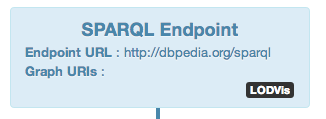
\includegraphics[width=55mm]{img/lodvis-int.png}
	\caption{LodVis integration link in a visualization of an analytical pipeline.}
	\label{fig:lodvis-int}
\end{figure}


\subsubsection{Visualising Payola data sources in LodVis}
With cooperation of the LodVis team, we have also implemented a reverse 
mechanism --- an API, which allows the user of the LodVis application to browse a 
dataset in the scope of the Payola application. To make it easy for the LodVis 
team to integrate a link to the Payola application, we prepared an API very 
similar to theirs. The URL pattern is very similar:

{  \scriptsize
\begin{verbatim}
http://live.payola.cz/visualize?endpointUri={endpoint-uri}&graphUri={graph-uri}
\end{verbatim}
}

In addition, we support referencing a list of graph URIs separated by a comma. Since 
we wanted to avoid any difficulties arising from passing a URI in an 
URL, we decided to have the parameters encoded with the Base64 algorithm.

The only problem was, that Payola was not able to visualize a dataset not registered
within its database. Therefore, when somebody accesses the 
URL, the application takes the parameters and creates an anonymous analyzer 
pipeline. The only plugin in the pipeline is a data source specified by the 
passed parameters. By evaluating such a pipeline, the user is able to visualize 
the neighbourhood of the vertex in the given dataset. The vertex is chosen by the 
SPARQL endpoint backend, e.g. OpenLink Virutoso~\cite{virtuoso}.

To allow an anonymous user to modify the pipeline, we also set a 
cookie with an authorization token to their browser. When logged into  
Payola a user with such a token can overtake the ownership of the pipeline and 
fully modify it.

\subsection{Secured endpoints}
What was also lacking was the support for password--guarded SPARQL endpoints. 
It is a natural matter, that a company would like to keep its statistics 
non--public, but they might wish to analyze and visualize them. Therefore, we 
have decided to introduce a support for secured endpoints.

Since every SPARQL endpoint may have different possible solutions, we have 
introduced a support for only one specific engine. We chose the most
used OpenLink Virutoso~\cite{virtuoso}.
It takes advantage of the Digest HTTP authentication as introduced in the 
RFC~2617~\cite{rfc-2617}. Therefore, we had to include the Apache HTTP commons 
library~\cite{apache-http-commons}. It was also necessary to introduce a new 
subtype of \texttt{string} parameter --- \texttt{password}. That was done as 
before (remember the \texttt{isMultiline} or the \texttt{isPattern} flag) by 
adding a new flag.

One can see a visualization of the described plugin in Figure~\ref{fig:secured-ds}. 

\begin{figure}
	\centering
	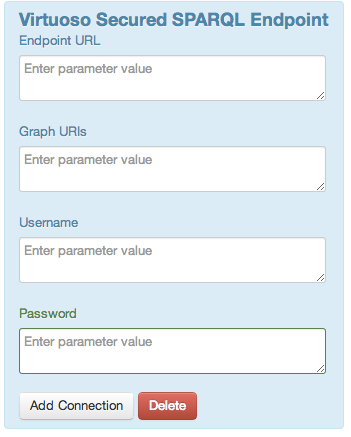
\includegraphics[width=55mm]{img/secured.png}
	\caption{One may simply include an instance of Virtuoso Secured SPARQL Endpoint plugin instead
	of an instance of the generic SPARQL Endpoint plugin.}
	\label{fig:secured-ds}
\end{figure}

\subsection{Analytical pipeline reuse}
During the period of writing this thesis Payola has undertaken a user test. One 
of the significant results of the test was that the users wished to modify the
analyses of others. At least, they would like to reference an analysis of 
another user within their own. That also fits into analyzing statistical data --- 
a company provides an analysis and presents its statistics while somebody else 
whishes to process them and apply DCV. That is why two different features 
were added.

\subsubsection{Clone and edit}
The first one is less powerful. It enables the user to clone an analysis of 
another user. After doing that, they get a newly created analysis owned by 
them. Therefore, they are in a full control of the analysis and may modify it in 
any way they want.

We were required to enhance the capabilities of the application in order to 
support cloning a plugin instance. We also had to clone bindings from an 
existing analytical pipeline and translate the identifiers of the cloned plugin 
instances in order to keep the bindings working.

The most difficult part was, unfortunately, to find a way of storing the cloned 
analysis, because the data access layer was not prepared for that. That is why
the persistence of the cloned analysis had to be split into several steps and may take a 
bit longer than expected.

As a result the user is presented with a inconspicuous button as shown in 
Figure~\ref{fig:clone-button}.

\begin{figure}
	\centering
	
\includegraphics[width=100mm]{img/clone-button.png}
	\caption{A clone button.}
	\label{fig:clone-button}
\end{figure}

\subsubsection{Inner analyses}
Much powerful feature is enabling the user to reference an existing analysis in 
another one. We introduced a fake analytical plugin with no implementation at 
all. It allows the user to insert a reference to an existing analysis instead 
of specifying a data source. As the inserted analysis generates a graph, 
it is hence a graph generator and might be considered a data source.

Of course, we had to find a way of implementing such a feature without 
making huge modifications of the evaluation framework. That is why the plugin 
has no implementation at all. The trick is that before starting an analysis 
evaluation we walk through the analysis and make some changes. The idea is very 
simple. We examine the analysis and replace each instance of the fake plugin 
with all the plugins from the referenced analysis. We call such a process an 
\emph{analysis expansion}.

To make the feature even more sophisticated we made a special user interface to 
enable them to parametrize an inner analysis. When inserting an analysis into 
another, the user is able to click the names of parameters of plugin instances 
in the inner analysis in order to promote them to \emph{analysis parameters}.

That is why we took an advantage of what we have learned while implementing the 
core of this thesis and created a special plugin for each inner analysis. That 
makes it possible for the plugin to have a variable parameters count. As a result the 
user creates a new shareable plugin. Such a plugin is also promoted to be a new 
data source available at any time in the future.

Moreover, we gave the user a tool for a simple parametrization of an existing analysis. 
They do not need to extend the analysis with other steps. They may simply take 
advantage of the new feature to ease their work.

\begin{figure}
	\centering
	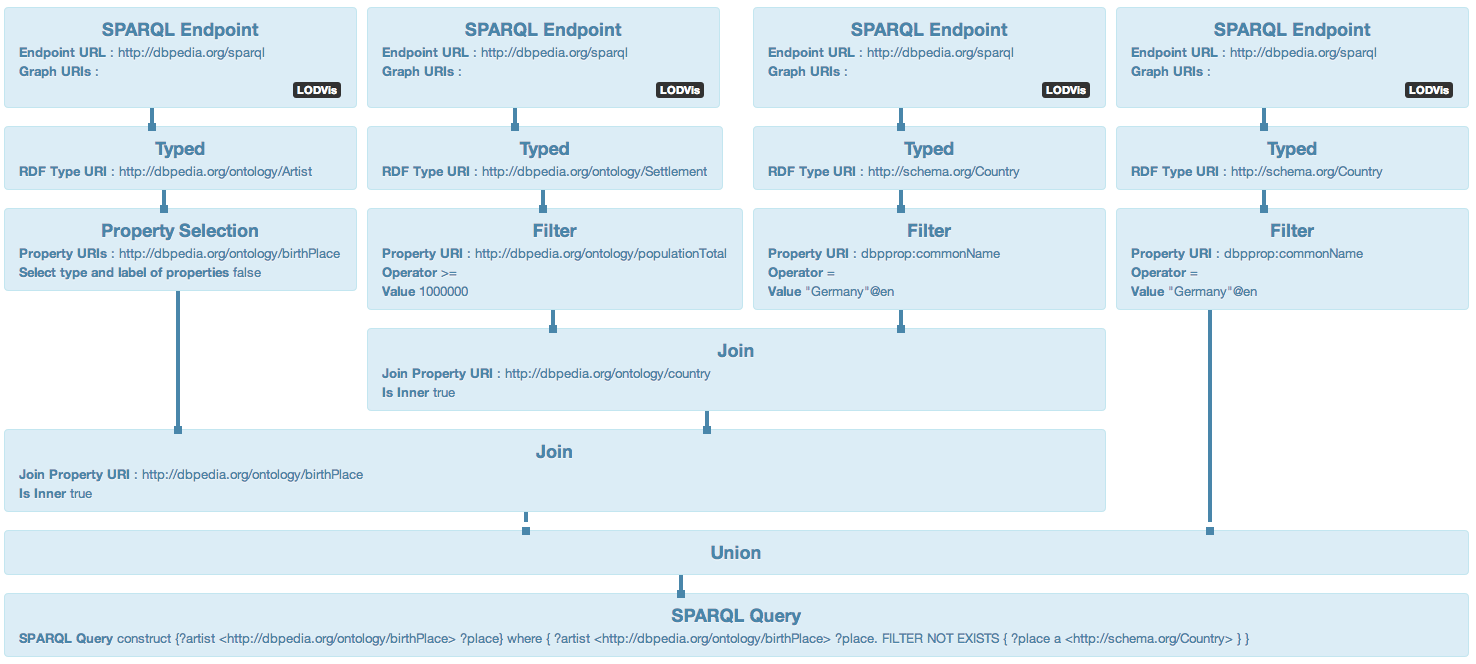
\includegraphics[width=140mm]{img/inner-example.png}
	\caption{A great example of an analysis that can benefit from inner analyses. Notice the
	two rightmost branches of the analytical pipeline. They are the same. By making
	an inner analysis we can at least convert the analysis into a pipeline shown in 
	Figure~\ref{fig:inner-example-simpler}}.
	\label{fig:inner-example}
\end{figure}

\begin{figure}
	\centering
	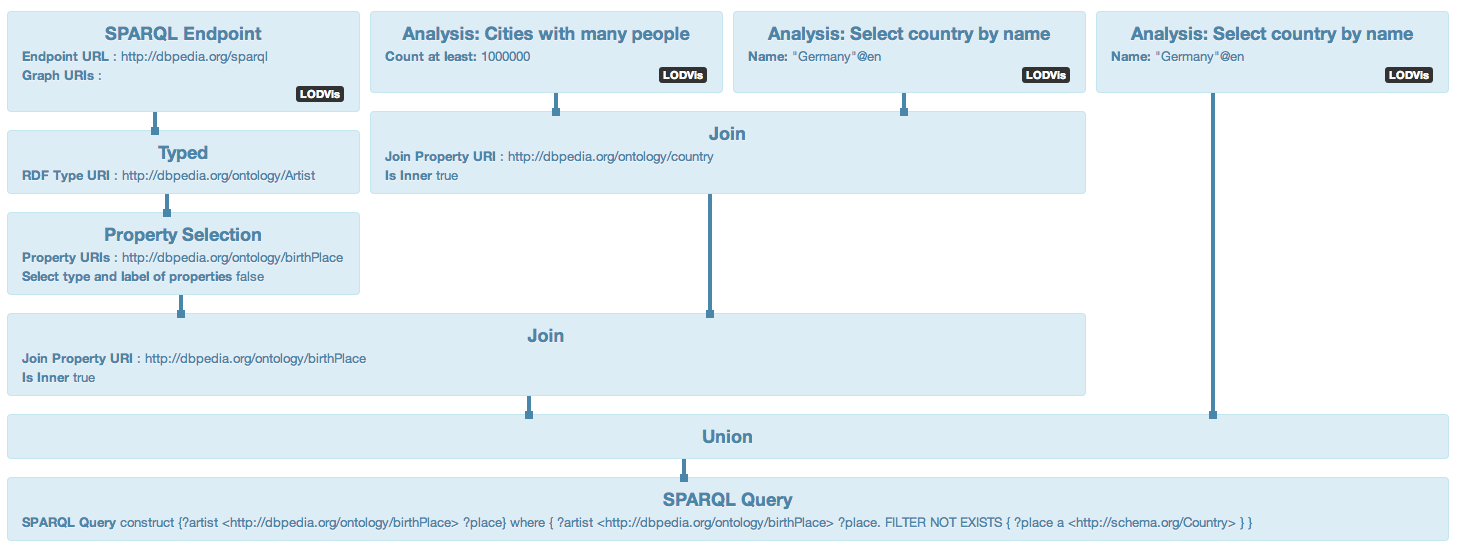
\includegraphics[width=140mm]{img/inner-example-simpler.png}
	\caption{An example of simplifying an analysis while utilizing inner analyses.}.
	\label{fig:inner-example-simpler}
\end{figure}

\subsection{Data Source browser permalinks}
Another minor change was done within the scope of the data source browser.
We introduced a mechanism, which enables to user to send a link to a current 
state of the triple table data source browser. It detects the specified URI in 
the URL and fetches an initial vertex based on that. The original behaviour delegates 
the decision on an underlying engine of the queried data source. We simply add a 
location hash to the URL that makes the permalink available in the address bar 
of the user's browser. The implementation was extended with a onload event 
handler, which looks for the location hash and reacts to it.

\subsection{Limit plugin}
In order to bring a better performance and user experience to the DataCube plugin
preview mechanism, we had to implement a completely new plugin. It is derived 
from the \texttt{ConstructQuery} class in order to allow some optimalizations. 
We needed to modify the \texttt{DataFetcher} plugin and introduce new 
optimalization phases to increase the speed of the most common cases of dataset 
preview. For instance, we merge a \texttt{DataFetcher} plugin followed by 
\texttt{Typed} and \texttt{Filter}, terminated with the \texttt{Limit} plugin 
into a single SPARQL query. We have also implemented a phase which optimizes
the query in the case we combine a common SPARQL query with the \texttt{Limit} plugin.
